%\documentclass[mathserif]{beamer}
\documentclass[handout]{beamer}
%\usetheme{Goettingen}
\usetheme{Warsaw}
%\usetheme{Singapore}
%\usetheme{Frankfurt}
%\usetheme{Copenhagen}
%\usetheme{Szeged}
%\usetheme{Montpellier}
%\usetheme{CambridgeUS}
%\usecolortheme{}
%\setbeamercovered{transparent}
\usepackage[utf8x]{inputenc} 
\usepackage[spanish]{babel} %idioma
\usepackage{amsmath, amssymb}
\usepackage{dsfont}
\usepackage{graphics}
\usepackage{cases}
\usepackage{graphicx}
\usepackage{pgf}
\usepackage{epsfig}
\usepackage{amssymb}
\usepackage{amstext}
\usepackage[ruled,vlined,lined]{algorithm2e}
\usepackage{amsmath}
\usepackage{epic}
\usepackage{epsfig}
\usepackage{fontenc}
\usepackage{palatino, url, multicol}
\usepackage{listings}
%\algsetup{indent=2em}
\newcommand{\factorial}{\ensuremath{\mbox{\sc Factorial}}}
\newcommand{\BIGOP}[1]{\mathop{\mathchoice%
{\raise-0.22em\hbox{\huge $#1$}}%
{\raise-0.05em\hbox{\Large $#1$}}{\hbox{\large $#1$}}{#1}}}
\newcommand{\bigtimes}{\BIGOP{\times}}
\vspace{-0.5cm}
\title{Introducción a R}
\vspace{-0.5cm}
\author[Felipe Bravo Márquez]{\footnotesize
%\author{\footnotesize  
 \textcolor[rgb]{0.00,0.00,1.00}{Felipe José Bravo Márquez}} 

%\vspace{-0.3cm}
%\institute{Universidad Técnica Federico Santa María - Diplomado Base de Datos}
\date{ \today }
%\logo{\includegraphics[height=1cm]{imagenes/dcc-small.png}}

\begin{document}
\begin{frame}
\titlepage


\end{frame}


%%%%%%%%%%%%%%%%%%%%%%%%%%%


\section{Introducción}

\begin{frame}{Motivación}

\scriptsize{
\begin{itemize}
 \item Diaramente se almacenan masivamente grandes colecciones de datos. 
 \item Ej: La Web, comercio electrónico, datos transaccionales.
 \item Los computadores se vuelven cada vez más baratos y con mayor poder de procesamiento.
 \item Analizar estos datos permite encontrar patrones ocultos. 
 \item Un buen uso de los datos puede traer beneficios de negocio. Ej: segmentación de clientes, predicción de demanda.
\end{itemize}

}
\begin{figure}[h!]
	\centering
	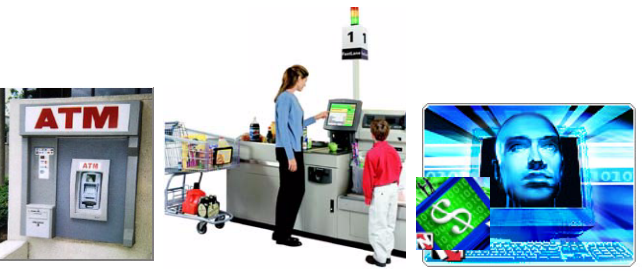
\includegraphics[scale=0.5]{imagenes/supermercado.png}
\end{figure}
 
\end{frame}


\begin{frame}{El proyecto R para la estadística computacional}
\begin{figure}[h!]
	\centering
	
\includegraphics[scale=0.6]{imagenes/Rlogo.png}
\end{figure}
\scriptsize{
\begin{itemize}
 \item R es un ambiente de programación estadístico totalmente gratuito: \url{http://www.r-project.org/}
 \item Permite manipular y almacenar datos de manera efectiva.
 \item Es un lenguaje de programación completo: variables, loop, condiciones, funciones.
 \item Provee muchas librerías para realizar distintos tipos de análisis sobre colecciones de datos, ej: visualización de datos, análisis de series temporales, análisis de grafos, análisis de texto.
 \item Las librerías junto a sus dependencias se encuentra ordenadas en un repositorio llamado \textbf{CRAN}: \url{http://cran.r-project.org/}

\end{itemize}

}



\end{frame}


\begin{frame}{¿Por qué usar R?}


\scriptsize{
\begin{itemize}
 \item R es software libre a diferencia de Matlab, SPSS, STATA.
 \item Esta disponible para muchos sistemas operativos: Windows, MAC OS X, Linux.
 \item Hasta el año 2013 la encuesta de \textbf{KDnuggets} mostraba a R como el lenguaje de programación preferido para realizar análisis de datos, minería de datos y ciencia de datos.
 \item \url{http://www.kdnuggets.com/2013/08/languages-for-analytics-data-mining-data-science.html}
 \item Hoy en día Python ha tomado mucha popularidad.
\end{itemize}

}

\begin{figure}[h!]
	\centering
	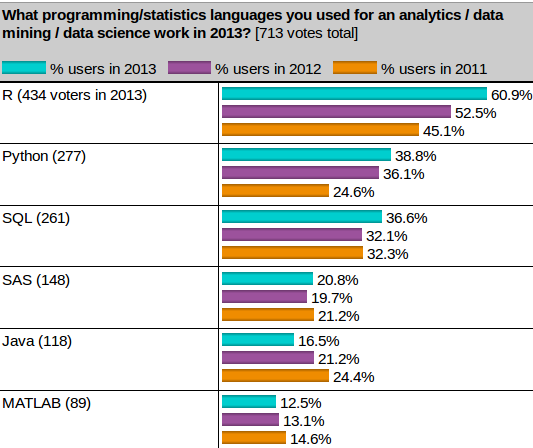
\includegraphics[scale=0.3]{imagenes/rpoll.png}
\end{figure}


\end{frame}

\begin{frame}{RStudio}
\scriptsize{
\begin{itemize}
 \item R funciona a través de la línea de comandos.
 \item Para trabajar en un entorno más amigable usaremos RStudio.
 \item También es gratis y se puede descargar para distintos sistemas operativos en este link: \url{http://www.rstudio.com/ide/download/desktop}
\end{itemize}

} 

\begin{figure}[h!]
	\centering
	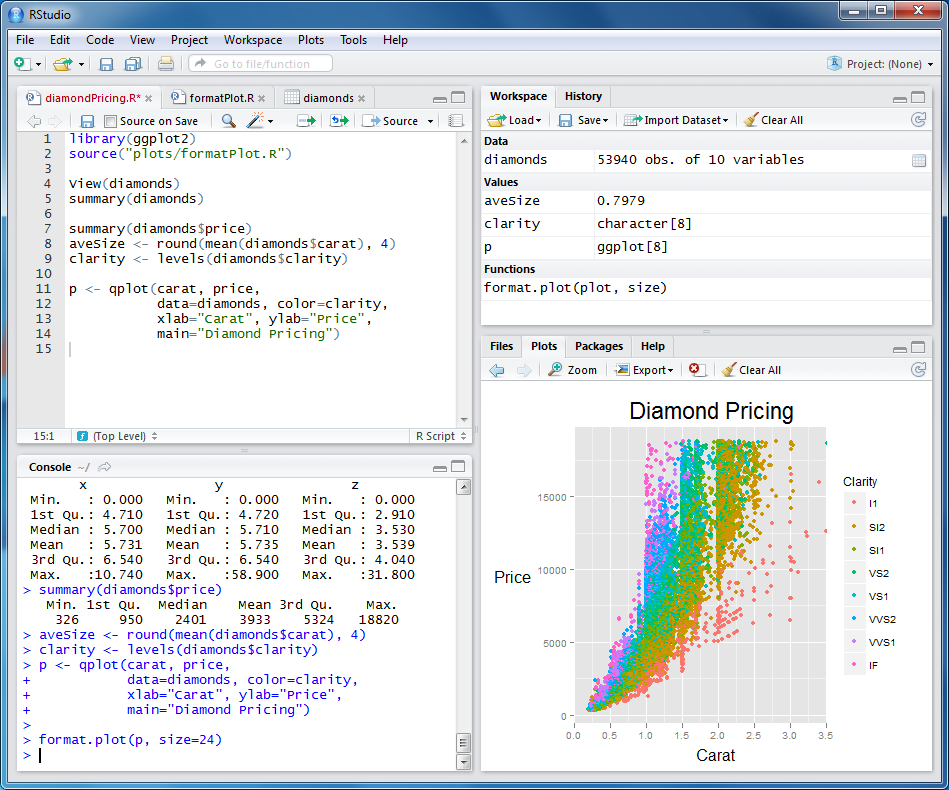
\includegraphics[scale=0.2]{imagenes/rstudio.png}
\end{figure}

 
\end{frame}


\section{Comandos básicos en R}

\begin{frame}[fragile]{R puede ser usado como una calculadora}
\begin{verbatim}
> 4*5
[1] 20
> 2^3
[1] 8
> exp(-5)
[1] 0.006737947
> log(4)
[1] 1.386294
\end{verbatim}


 
\end{frame}




\begin{frame}[fragile]{Declarando Variables}
\scriptsize{
\begin{itemize}
 \item Las variables se pueden asignar usando \verb+<-+ , \verb+=+ o la función \verb+assign+ 
 
  \begin{verbatim}
a<-1
b=3
assign("tres",3)
d<-a+b
ver<-T # equivalente a TRUE
pal<-"hola"
\end{verbatim}
 
 \item Por convención usamos la primera forma (\verb+<-+).
 
\item Las variables pueden ser de clase \textbf{numeric}, \textbf{factor}, \textbf{character}, \textbf{logical}, entre otras.
 
\item Para ver el tipo de una variable usamos el comando \verb+class+.
 \begin{verbatim}
  > class(a) 
[1] "numeric"
> class(ver)
[1] "logical"
> class(pal)
[1] "character"
 \end{verbatim}

 
 
\end{itemize}

}


\end{frame}


\begin{frame}[fragile]{Funciones}
\scriptsize{
\begin{itemize}
 \item Las funciones se declaran como variables y se crean con la expresión \textbf{function}:

\begin{verbatim}
suma<-function(a=2,b=1){
  a+b;
}

fac<-function(n){
  ifelse(n==1,return(1),return(n*fac(n-1)))    
}

\end{verbatim}

\item Los parámetros de la función se pueden declaran con un valor específico para usarlos como valores predeterminados cuando no entregamos valores para esos parámetros:
\begin{verbatim}
> suma(3,4)
[1] 7
> suma()
[1] 3
 
\end{verbatim}

\item Las funciones son del tipo \textbf{function}:
\begin{verbatim}
> class(suma)
[1] "function" 
\end{verbatim}


\end{itemize}


 
} 
\end{frame}

\begin{frame}[fragile]{Ayuda y el Workspace}
\scriptsize{
\begin{itemize}
 \item Para leer documentación sobre una función usamos \textbf{help} o \textbf{?}:
\begin{verbatim}
help(ls)
?ls
#Para un comando particular
help("for")

\end{verbatim}

\item Todas las variables quedan en mi ambiente \textbf{workspace}. Para listarlos se usa el comando \textbf{objects} o \textbf{ls}. Para borrar una variable usamos \textbf{rm}:

\begin{verbatim}
objects()
ls()
rm(a)
#Para borrarlos todos
rm(list=ls())
 
\end{verbatim}


\item Puedo grabar todas mis variables de workspace en un archivo y así recuperar mi trabajo en una sesión futura:
\begin{verbatim}
save.image("myworkspace.RData")
#Luego lo cargamos
load("myworkspace.RData")
 
\end{verbatim}


 
 
 
 \end{itemize}



}
 
 
\end{frame}

\begin{frame}[fragile]{Vectores}
\scriptsize{
\begin{itemize}
 \item Para trabajar con colecciones de elementos declaramos \textbf{vectores} que se construyen con el comando \textbf{c}:
 \begin{verbatim}
edades<-c(21,33,12,34,23,70,90,80,7,29,14,2,
          88,11,55,24,13,11,56,28,33)
 \end{verbatim}
 \item Para obtener el largo de un vector usamos el comando \textbf{length}, luego para obtener la suma de todos los elementos usamos \textbf{sum}:
 \begin{verbatim}
> suma<-sum(edades)
> largo<-length(edades)
> suma
[1] 734
> largo
[1] 21
 \end{verbatim}
 
\item Si operamos un vector por un escalar este valor se recicla para todos los elementos del vector:
 \begin{verbatim}
> numeros<-c(1,2,3)
> numeros+3
[1] 4 5 6
> numeros*5
[1]  5 10 15
 \end{verbatim}
\end{itemize}




}
 
 
\end{frame}

\begin{frame}[fragile]{Vectores (2)}
\scriptsize{
\begin{itemize}
 \item Calcular la media y la varianza del vector edades usando los comandos \textbf{sum} y \textbf{length} en base a las siguientes ecuaciones:
 \begin{equation}
  \text{media}(\text{edades})=\frac{\sum_{i=1}^n\text{edades}_{i}}{n}
 \end{equation}
 
 \begin{equation}
 \text{varianza}(\text{edades})=\frac{\sum_{i=1}^n(\text{edades}_{i}-\text{media}(\text{edades}))^2 }{n-1} 
 \end{equation}

 
\end{itemize}



}

 
\end{frame}



\begin{frame}[fragile]{Vectores (4)}
\scriptsize{
\begin{itemize}
 \item Respuesta:
 \begin{verbatim}
> media<-sum(edades)/length(edades)
> media
[1] 34.95238
> varianza<-sum((edades-media)^2)/(length(edades)-1)
> varianza
[1] 747.9476
 \end{verbatim}
 
 \item R dispone de funciones \textbf{mean} y \textbf{var}:
 \begin{verbatim}
> mean(edades)
[1] 34.95238
> var(edades)
[1] 747.9476

 \end{verbatim}
 
\end{itemize}



}

 
\end{frame}
 
 
\begin{frame}[fragile]{Vectores (5)}
\scriptsize{
\begin{itemize}
 
\item Cuando construimos vectores con elementos de distinto tipo, R los convierte todos a un tipo único:
\begin{verbatim}
> c("hola",2,T)
[1] "hola" "2"    "TRUE"
> c(TRUE,FALSE,500)
[1]   1   0 500 
\end{verbatim}

 \item Los elementos de un vector pueden se declarados con nombres para luego recuperarlos con el comando \textbf{names}:
\begin{verbatim}
> notas<-c(Juan=4.5,Luis=6.2,Romina=3.9,Felipe=2.8,Mariana=6.7)
> names(notas)
[1] "Juan"    "Luis"    "Romina"  "Felipe"  "Mariana"
 
\end{verbatim}
\item Podemos ordenar un vector usando el comando \textbf{sort}:
\begin{verbatim}
> names(sort(x=notas,decreasing=T))
[1] "Mariana" "Luis"    "Juan"    "Romina"  "Felipe" 
\end{verbatim}

\end{itemize}



}
\end{frame}

\begin{frame}[fragile]{Acceso  Vectores}
\scriptsize{
\begin{itemize}

 \item R permite acceder a los elmentos de un vector por medio de índices numéricos \verb+[i]+: 
\begin{verbatim}
> notas[1] # primer elemento
Juan 
 4.5
\end{verbatim}

\item El índice puede ser otro vector númerico para acceder a más de un elemento:
\begin{verbatim}
> notas[c(1,5)] # primer y quinto elemento
   Juan Mariana 
    4.5     6.7 
\end{verbatim}

\item Si queremos omitir algún elemento usamos índices negativos:
\begin{verbatim}
> notas[-2] # Todos menos el segundo
   Juan  Romina  Felipe Mariana 
    4.5     3.9     2.8     6.7 
\end{verbatim}

\item También se pueden acceder a los elementos por sus nombres:
\begin{verbatim}
> notas[c("Juan","Mariana")] # Sólo Juan y Mariana
   Juan Mariana 
    4.5     6.7 
\end{verbatim}



\end{itemize}

 

 }
\end{frame}


\begin{frame}[fragile]{Operando Vectores}
\scriptsize{
\begin{itemize}
 \item Vimos anteriormente que si opero un escalar por un vector, el escalar se aplica a todos los elementos del vector.
 \item Si tengo ahora dos vectores del mismo largo y los opero, la operación se hace elemento por elemento:
\begin{verbatim}
a<-c(1,2)
b<-c(3,4)
> a+b
[1] 4 6
> a*b
[1] 3 8
\end{verbatim}

\end{itemize}
 }
\end{frame}



\begin{frame}[fragile]{Operando Vectores (2)}
\scriptsize{
\begin{itemize}
\item Si los vectores son de largo distinto, el más pequeño recicla sus elementos:
\begin{verbatim}
> d<-c(4,5,6,9)
> a+d
[1]  5  7  7 11
> c(a,a)+d
[1]  5  7  7 11
\end{verbatim}

\item Si el largo del mayor no es múltiplo del largo del menor, recibimos una advertencia:
\begin{verbatim}
> c(1,2)+c(-9,2,3)
[1] -8  4  4
Warning message:
In c(1, 2) + c(-9, 2, 3) :
  longer object length is not a multiple of shorter object length 
\end{verbatim}
 
\end{itemize}
 }
\end{frame}



\begin{frame}[fragile]{Comparando Vectores}
\scriptsize{
\begin{itemize}
 \item R soporta los operadores de comparación para variables numéricas:\verb+>,<, ==, <=, >=, !=+ además de \verb+& |+ como los operadores \textbf{and} y \textbf{or} para variables lógicas:
\begin{verbatim}
> menores<-edades<18
> menores
 [1] FALSE FALSE  TRUE FALSE FALSE FALSE FALSE FALSE  TRUE FALSE  TRUE  TRUE FALSE  TRUE FALSE FALSE
[17]  TRUE  TRUE FALSE FALSE FALSE
\end{verbatim}
\item Si le damos a un vector un índice de variables lógicas recuperamos los valores donde el índice toma el valor verdadero: 
\begin{verbatim}
> edades[menores] 
[1] 12  7 14  2 11 13 11
\end{verbatim}

\item Ejercicio: calcular el promedio de edad de los elementos mayores o iguales a 18 años. 
\begin{verbatim}
mean(edades[edades>=18]) 
\end{verbatim}

 
\end{itemize}



}
\end{frame}

\begin{frame}[fragile]{Valores Nulos}
\scriptsize{
\begin{itemize}
\item En R, los valores faltantes se escriben como \verb+NA+. Es común que aparezcan cuando leemos datos de alguna base de datos. Algunas funciones no aceptan valores nulos por lo que hay que tenerlos en cuenta.
\begin{verbatim}
> missing_vector<-c(12,15,NA)
> missing_vector
[1] 12 15 NA
\end{verbatim}

\item Para chequear si una variable es nula usamos el comando \verb+is.na+:
\begin{verbatim}
> missing_vector[!is.na(missing_vector)]
[1] 12 15 
\end{verbatim}



\end{itemize}

 }
 
 
\end{frame}




\begin{frame}[fragile]{Secuencias}
 \scriptsize{
 
 \begin{itemize}
  \item Para crear un vector formado por una secuencia de números usamos el comando \textbf{seq}:
 
 \begin{verbatim}
> pares<-seq(from=2,to=20,by=2)
> cuatro_mult<-seq(from=4,by=4,length=100)
> pares
 [1]  2  4  6  8 10 12 14 16 18 20
 \end{verbatim} 
 \item También se pueden crear usando el operador (\verb+:+):
 \begin{verbatim}
> 1:10
 [1]  1  2  3  4  5  6  7  8  9 10 
> seq(1,10,1)
 [1]  1  2  3  4  5  6  7  8  9 10
 \end{verbatim} 
 \end{itemize}
 
 }
\end{frame}

\begin{frame}[fragile]{Repeticiones}
\scriptsize{
\begin{itemize}
 \item Para crear vectores que repitan un valor u otro vector varias veces usamos el comando \textbf{rep}. El primer valor es el objeto a repetir y el segundo es el número de repeticiones:
 \begin{verbatim}
> rep(10,3)
[1] 10 10 10
> rep(c("hola","chao"),4)
[1] "hola" "chao" "hola" "chao" "hola" "chao" "hola" "chao"
 \end{verbatim}
 \item Problema: Crear una secuencia que repita 3 veces los 4 primeros múltiplos de 7. \pause
 \begin{verbatim}
> rep(seq(from=7,by=7,length=4),3)
 [1]  7 14 21 28  7 14 21 28  7 14 21 28
\end{verbatim}
 
 
\end{itemize}
 
 
 
} 
\end{frame}

\begin{frame}[fragile]{Generación de vectores aleatorios}
\scriptsize{
\begin{itemize}
 \item Para realizar experimentos o simular fenómenos de comportamiento conocido es muy útil generar vectores aleatorios. 
 \item Si queremos números uniformemente distribuidos entre un máximo y un mínimo usamos \textbf{runif}:
 \begin{verbatim}
> runif(n=5, min = 1, max = 10)
[1] 5.058862 1.737830 9.450956 9.149376 2.652774
 \end{verbatim}
 \item Si queremos números centrados en una media $\mu$ y con una desviación estándar $\sigma$, usamos una distribución normal con \textbf{rnorm} donde sabemos que el $68\%$ de las observaciones estarán alrededor $\mu\pm\sigma$, el $95\%$ en $\mu\pm2\sigma$ y el $99.7\%$ en $\mu\pm3\sigma$:
 
 \begin{verbatim}
> rnorm(n=5, mean = 10, sd = 4)
[1] 12.081286  2.636001 16.001953  0.120463  6.211835
 \end{verbatim}
 
\end{itemize}

}
\end{frame}

\begin{frame}[fragile]{Generación de vectores aleatorios (2)}
\scriptsize{
\begin{itemize}
 \item Cuando queremos modelar un número de arribos por unidad de tiempo para simular modelos de colas, usamos la distribución de \textbf{Poisson} con \textbf{rpos}. El parámetro $\lambda$ nos dice la cantidad promedio de llegadas en un período:
 \begin{verbatim}
> rpois(n=10, lambda = 3)
 [1] 1 3 8 6 1 1 6 3 4 7
 \end{verbatim}

 \item Un experimento de distribución binomial se basa en tener $n$ experimentos, donde en cada experimento  realizamos $k$ intentos de un fenómeno cuya probabilidad de acierto en cada intento es $p$. Con el comando \textbf{rbinom} podemos simular la cantidad de aciertos obtenidos en cada experimento.
\begin{verbatim}
> rbinom(n=10,size=2,prob=0.5)
 [1] 0 1 2 1 1 0 2 0 0 1
> rbinom(n=10,size=2,prob=0.7)
 [1] 1 2 2 1 0 1 2 2 2 2
> rbinom(n=10,size=2,prob=0.2)
 [1] 0 0 0 0 1 0 1 0 1 0 
\end{verbatim}

 
 
\end{itemize}


}
\end{frame}


\begin{frame}[fragile]{Variables Categóricas o Factores}
\scriptsize{
\begin{itemize}
 \item Además de las variables numéricas o lógicas, se puede trabajar con variables categóricas. Ej: color, sexo, clase social.
 \item Se crean con el comando \textbf{factor} y los posibles valores de la variable se guardan en el atributo \textbf{levels}.
\begin{verbatim}
> gente<-factor(c("Hombre","Mujer","Mujer","Mujer","Hombre"))
> gente
[1] Hombre Mujer  Mujer  Mujer  Hombre
Levels: Hombre Mujer
> class(gente)
[1] "factor"
> levels(gente)
[1] "Hombre" "Mujer" 
#Puedo renombrar a los niveles
> levels(gente)<-c("Man","Woman")
> gente
[1] Man   Woman Woman Woman Man  
Levels: Man Woman
\end{verbatim}
 
\end{itemize}

}
\end{frame}


\begin{frame}[fragile]{Agregando variables por categorías con \textbf{tapply}}
\scriptsize{
\begin{itemize}
 \item Si tenemos un vector numérico y otro categórico del mismo largo podemos aplicar una función de agregación.
 \item Ejemplo: Creo una categoría para el vector edades de niveles \emph{niño}, \emph{adolescente}, \emph{adulto}:
 \begin{verbatim}
categ_edades<-ifelse(edades<12,"niño",
                      ifelse(edades<18,"adolescente","adulto"))
class(categ_edades)
[1] "character"
#Convierto a factor con as.factor
categ_edades<-as.factor(categ_edades)
 \end{verbatim}

 \item Ahora cuento la cantidad de personas por categoría, y calculo la media y la desviación estándar para cada grupo:
\begin{verbatim}
tapply(edades,categ_edades,length)
adolescente      adulto        niño 
          3          14           4 
> tapply(edades,categ_edades,mean)
adolescente      adulto        niño 
   13.00000    47.42857     7.75000 
> tapply(edades,categ_edades,sd)
adolescente      adulto        niño 
   1.000000   25.294312    4.272002 
  
\end{verbatim}

 
\end{itemize}



}
\end{frame}


\begin{frame}[fragile]{Manejo de Strings}
\scriptsize{
 \begin{itemize}
  \item Puedo imprimir un string usando el comando \textbf{cat}:
\begin{verbatim}
> saludo<-"Hola Mundo"
> cat(saludo)
Hola Mundo
\end{verbatim}

\item Para concatenar dos strings uso el comando \textbf{paste}:
\begin{verbatim}
> paste("Hola","Chao",sep="-")
[1] "Hola-Chao"
> paste("persona",1:4, sep="")
[1] "persona1" "persona2" "persona3" "persona4"
> paste(saludo,1:3, sep=" ")
[1] "Hola Mundo 1" "Hola Mundo 2" "Hola Mundo 3" 
\end{verbatim}

\item Para extraer sub-cadenas usamos el comando \textbf{substr}:
\begin{verbatim}
> substr(saludo,1,4)
[1] "Hola" 
\end{verbatim}

\item Existe un vector llamado \textbf{letters} que tiene todas las letras del abecedario, útil para nombrar variables:
\begin{verbatim}
> letters[1:4]
[1] "a" "b" "c" "d" 
\end{verbatim}


 \end{itemize}

 }
\end{frame}


\begin{frame}[fragile]{Matrices}
\scriptsize{
 \begin{itemize}
  \item Las matrices son vectores de dos dimensiones. Por defecto se van llenando por columna:
 \begin{verbatim}
> matriz_por_col<-matrix(data=1:12,nrow=3,ncol=4)
> matriz_por_col
     [,1] [,2] [,3] [,4]
[1,]    1    4    7   10
[2,]    2    5    8   11
[3,]    3    6    9   12 
 \end{verbatim}
 \item Para llenarlas por fila uso el parámetro \textbf{byrow}:
 \begin{verbatim}
> matriz_por_fil<-matrix(data=1:12,nrow=4,ncol=3,byrow=T)
> matriz_por_fil
     [,1] [,2] [,3]
[1,]    1    2    3
[2,]    4    5    6
[3,]    7    8    9
[4,]   10   11   12  
 \end{verbatim}

 \item Accedemos a la dimensión de la matriz con el comando \textbf{dim}.
 \begin{verbatim}
 > dim(matriz_por_fil)
[1] 4 3 
 \end{verbatim}

 \end{itemize} 
 }
\end{frame}


\begin{frame}[fragile]{Matrices (2)}
\scriptsize{
 \begin{itemize}
  \item Para acceder a los elementos de una matriz tengo que especificar las filas $i$ y las columnas $j$ \verb+[i,j]+. Si dejo alguno de los dos valores vacío se recuperan todos las filas o columnas: 
 \begin{verbatim}
 > matriz_por_fil[2,] #Segunda fila, todas las columnas
[1] 4 5 6
> matriz_por_fil[2,1] # Segunda fila, primera columna
[1] 4
> matriz_por_fil[-1,-2] # Descarto fila 1 y columna 2
     [,1] [,2]
[1,]    4    6
[2,]    7    9
[3,]   10   12 
 \end{verbatim}
\item Para acceder a los nombres de las filas o columnas usamos \textbf{rownames} y \textbf{colnames} de forma análoga a como usamos \textbf{names} para los vectores.
\begin{verbatim}
> rownames(matriz_por_fil)<-paste("r",1:4,sep="")
> colnames(matriz_por_fil)<-paste("c",1:3,sep="")
> matriz_por_fil["r2","c3"]
[1] 6
\end{verbatim}  
 \end{itemize}
 }
\end{frame}


\begin{frame}[fragile]{Matrices (3)}
\scriptsize{
\begin{itemize}
 \item Puedo agregarle nuevas filas o nuevas columnas a una matriz usando \textbf{rbind} y \textbf{cbind} respectivamente:
 \begin{verbatim}
  > rbind(matriz_por_fil,r5=1:3)
   c1 c2 c3
r1  1  2  3
r2  4  5  6
r3  7  8  9
r4 10 11 12
r5  1  2  3
> cbind(matriz_por_fil,c4=4:1)
   c1 c2 c3 c4
r1  1  2  3  4
r2  4  5  6  3
r3  7  8  9  2
r4 10 11 12  1
 \end{verbatim}

\end{itemize}
 
 
 
} 
\end{frame}

\begin{frame}[fragile]{Matrices (4)}
\scriptsize{
\begin{itemize}
 \item Operaciones algebraicas como la multiplicación de matrices se hace con \verb+%*%+:
 \begin{verbatim}
>a<-matriz_por_col %*% matriz_por_fil
      c1  c2  c3
[1,] 166 188 210
[2,] 188 214 240
[3,] 210 240 270
 \end{verbatim}

 
\item  Si usamos solamente el operador \verb+*+, la multiplicación se hace elemento por elemento (sólo para matrices de igual dimensión). Esto aplica también para la suma, la resta, la división y otro tipo de operadores.

\end{itemize}


 
}

\end{frame}

\begin{frame}[fragile]{Matrices (5)}
\scriptsize{
\begin{itemize}
\item Podemos transponer una matriz con \textbf{t}:
 \begin{verbatim}
> t(a)
   [,1] [,2] [,3]
c1  166  188  210
c2  188  214  240
c3  210  240  270
\end{verbatim}
\item Los valores y vectores propios se calculan con \textbf{eigen}:
\begin{verbatim}
> eigen(a)
$values
[1] 6.483342e+02 1.665808e+00 3.437970e-14

$vectors
           [,1]        [,2]       [,3]
[1,] -0.5045331 -0.76077568  0.4082483
[2,] -0.5745157 -0.05714052 -0.8164966
[3,] -0.6444983  0.64649464  0.4082483
 \end{verbatim}

\end{itemize}


 
}

\end{frame}

\begin{frame}[fragile]{Arreglos o Tensores}
\scriptsize{
\begin{itemize}
 \item Los arreglos (o tensores) son como las matrices pero de más dimensiones:
 \begin{verbatim}
> arreglo<-array(1:8, dim=c(2,2,2))
> arreglo
, , 1

     [,1] [,2]
[1,]    1    3
[2,]    2    4

, , 2

     [,1] [,2]
[1,]    5    7
[2,]    6    8

> arreglo[1,2,1]
[1] 3
 \end{verbatim}

\end{itemize}


}
\end{frame}




\begin{frame}[fragile]{Listas}
\scriptsize{
\begin{itemize}
 \item Las matrices me restringen a que todos los vectores sean del mismo largo y del mismo tipo.
 \item Las listas me permiten agrupar objetos de cualquier tipo y de cualquier largo:
 \begin{verbatim}
milista<-list(hombre="Pepe",mujer="Juana",
              hijos=3,edades=c(4,8,12))
 \end{verbatim}
 \item Cuando accedo a sus elementos usando \verb+[i]+ recupero una sub-lista:
 \begin{verbatim}
> milista[c(3,4)] # Sublista
$hijos
[1] 3
$edades
[1]  4  8 12
 \end{verbatim}
\item Para acceder a una elemento particular tengo tres opciones:
\begin{verbatim}
milista[[1]]
milista[["hombre"]]
milista$hombre

[1] "Pepe"
\end{verbatim}


\end{itemize}



}
\end{frame}

\begin{frame}[fragile]{Ejercicio Lista}
\scriptsize{

\begin{itemize}
 \item Crear una lista que tenga tres vectores de largo 100  generado por alguno de los mecanismos vistos para generar vectores aleatorios. Pueden variar las distribuciones o los parámetros. Asígnele nombres a cada uno de los vectores. \pause
 \begin{verbatim}
 vectores<-list(normal=rnorm(n=100,mean=10,sd=5),
               poisson=rpois(n=100,lambda=10),
               uniforme=runif(n=100,min=5,max=15))
 \end{verbatim}

\item Calcule la media y la desviación estándar de cada uno de los vectores de la lista. \pause
\begin{verbatim}
medias<-vector()
desv<-vector()
for(i in 1:length(vectores)){
  medias[i]<-mean(vectores[[i]])
  desv[i]<-sd(vectores[[i]])
}
> medias
[1] 10.589222 10.390000  9.579866
> desv
[1] 5.155478 2.711349 2.905810
\end{verbatim}

 
\end{itemize}

}
\end{frame}

\begin{frame}[fragile]{Cálculos agregados a Listas con \textbf{sapply} y \textbf{lapply}}
 \scriptsize{
 \begin{itemize}
  \item El ejercicio anterior se puede resolver de manera mucho más sencilla en R con unas funciones especiales para realizar agregación sobre listas.
  \item El comando \textbf{sapply} permite aplicar una función a cada elemento de una lista y devuelve los resultados en un vector. Luego \textbf{lapply} hace lo mismo pero retorna una lista:
 \begin{verbatim}
 > sapply(vectores,mean)
   normal   poisson  uniforme 
10.589222 10.390000  9.579866 
> sapply(vectores,sd)
  normal  poisson uniforme 
5.155478 2.711349 2.905810  
 \end{verbatim}  

 \item Ejercicio, programar una propia versión de \textbf{sapply}. Hint: En R una funciones puede recibir otra  función como parámetro y aplicarla de manera genérica. \pause
\begin{verbatim}
 myapply<-function(lista,fun,...){
  resultado<-vector(length=length(lista))
  for(i in 1:length(lista)){
    resultado[i]<-fun(lista[[i]],...)
  }
  resultado  
}
\end{verbatim}
  
 \end{itemize}
 
 }
\end{frame}


\begin{frame}[fragile]{Data Frames}
\scriptsize{
\begin{itemize}
 \item El data.frame es el tipo de colección de datos más utilizada para trabajar con datasets en R.
 
 \item Un data.frame se compone de varios vectores, donde cada vector puede ser de distintos tipos, pero del mismo largo. Es equivalente a una tabla de una base de datos:
 \begin{verbatim}
edades.frame<-data.frame(edad=edades,categoria=categ_edades)

> edades.frame
   edad   categoria
1    21      adulto
2    33      adulto
3    12 adolescente
\end{verbatim}

\item Las dimensiones de un data.frame se acceden de la misma manera que en una matriz:
\begin{verbatim}
> length(edades.frame)
[1] 2
> dim(edades.frame)
[1] 21  2 
\end{verbatim}
 
\end{itemize}



}
\end{frame}

\begin{frame}[fragile]{Data Frames (2)}
\scriptsize{ 
\begin{itemize}
 \item Puedo acceder a los elementos como si fuese una matriz o una lista:
 \begin{verbatim}
> edades.frame[3,1] # La edad del tercer elemento
[1] 12
> edades.frame$edad[1:6] # La edad de los primeros 6 elementos
[1] 21 33 12 34 23 70
 \end{verbatim}
 
\item También puede pasar cada variable del data.frame a mi workspace con el comando \textbf{attach} y así accederlas directamente:
\begin{verbatim}
attach(edades.frame)
> categoria[1:3]
[1] adulto      adulto      adolescente
Levels: adolescente adulto niño
\end{verbatim}

\item Puedo guardar un data.frame en un archivo csv (separado por comas u otra carácter) usando \textbf{write.table}:
\begin{verbatim}
write.table(x=edades.frame,file="edades.csv",sep=",",row.names=F) 
\end{verbatim}

\item Pongo \verb+row.names=F+ para que no ponga los nombres de las columnas en el archivo.

 
\end{itemize}
 
}
\end{frame}


\begin{frame}[fragile]{Cargando Data Frames}
\scriptsize{
\begin{itemize}
 \item Puedo leer un data.frame desde archivos \textbf{csv} de manera nativa y desde otras fuentes (Excel, base de datos, etc.) usando librerías especiales:
 \begin{verbatim}
  my.frame<-read.table(file="edades.csv",header=T,sep=",")
 \end{verbatim}
\item El parámetro \verb+header+ específica si quiero usar la primera fila para asignarle nombres a las columnas.

\item Además R provee varias colecciones de datos para experimentar. Se pueden ver como el comando \verb+data()+.

\item Para ver todos los datasets disponibles de todas las librerías:
\begin{verbatim}
data(package = .packages(all.available = TRUE)) 
\end{verbatim}

\item Ahora podemos cargar un dataset, que se incluye como data.frame en mi workspace:
\begin{verbatim}
data(USArrests) # Arrestos en Estados Unidos por estado 
\end{verbatim}

 
\end{itemize}



}
\end{frame}



\begin{frame}[fragile]{Muestreo}
\scriptsize{
\begin{itemize}
 \item Cuando tenemos datasets muy grandes algunas técnicas estadísticas o de visualización pueden ser muy costosas computacionalmente.
 \item Se puede trabajar con una muestra aleatoria de los datos. 
 
 \item La idea es que si la muestra es representativa, la propiedades observadas serán equivalentes a las de la población.  
 
 \item En R se realiza el muestreo con el comando \textbf{sample}.
 
 \item Si la muestra es sin reemplazo, sacamos datos de manera aleatoria sin reponer el elemento. Entonces la muestra debe ser de menor tamaño que el dataset:

 \begin{verbatim}
> sample(edades,size=4,replace=F)
[1] 80 88 12 23
\end{verbatim}
\end{itemize}



}
\end{frame}


\begin{frame}[fragile]{Muestreo (2)}
\scriptsize{
\begin{itemize}
 \item Si la muestra es con reemplazo poddemos observar datos duplicados. De esta forma, la muestra puede ser incluso de mayor tamaño que la colección original: 

\begin{verbatim}
sample(edades,size=100,replace=T)
\end{verbatim}
 
 \item Cuando tenemos que los datos vienen etiquetados por alguna categoría y tomamos una muestra donde cada categoría tiene una participación proporcional a la de la colección original, tenemos un muestreo estratificado. 
 
 \item Ejercicio: extraer una muestra aleatoria sin reemplazo que tenga 10 filas del data.frame \textbf{USArrests}. \pause
 
 \begin{verbatim}
 USArrests[sample(1:(dim(USArrests)[1]),size=10,replace=F),]
 \end{verbatim}

\end{itemize}



}
\end{frame}






\begin{frame}[fragile]{Instalando librerías adicionales}
\scriptsize{
\begin{itemize}
 \item R tiene una comunidad muy activa que desarrolla muchas librerías para el análisis y la visualización de datos.
 \item Se pueden descargar librerías adicionales desde el repositorio CRAN directamente desde R.
 \item Las librerías se pueden instalar desde Rstudio o con el siguiente comando:
 \begin{verbatim}
 install.packages("rpart",dependencies=T)
\end{verbatim} 

\item Luego para poder usarlas se cargan de la siguiente forma: \verb+library(rpart)+.

\item Un conjunto de liberías muy útiles para manipular datos es \textit{tydyverse}:  \url{https://www.tidyverse.org/}.

 \begin{verbatim}
install.packages("tidyverse")
\end{verbatim} 


 
 \end{itemize}

 
}
 
\end{frame}



%%%%%%%%%%%%%%%%%%%%%%%%%%%
\begin{frame}[allowframebreaks]\scriptsize
\frametitle{Bilbiografía}
%\bibliography{bio}
%\bibliographystyle{apalike}
\begin{thebibliography}{8}

\bibitem{William}
Venables, William N., David M. Smith, and R Development Core Team. \emph{An introduction to R.}, 2002.
\end{thebibliography}


%\bibliographystyle{flexbib}
\end{frame}




%%%%%%%%%%%%%%%%%%%%%%%%%%%

\end{document}
